\documentclass{standalone}
\usepackage{tikz}
\usetikzlibrary{patterns, positioning}
\usepackage[sfdefault]{ClearSans} %% option 'sfdefault' activates Clear Sans as the default text font
\usepackage[T1]{fontenc}

\begin{document}
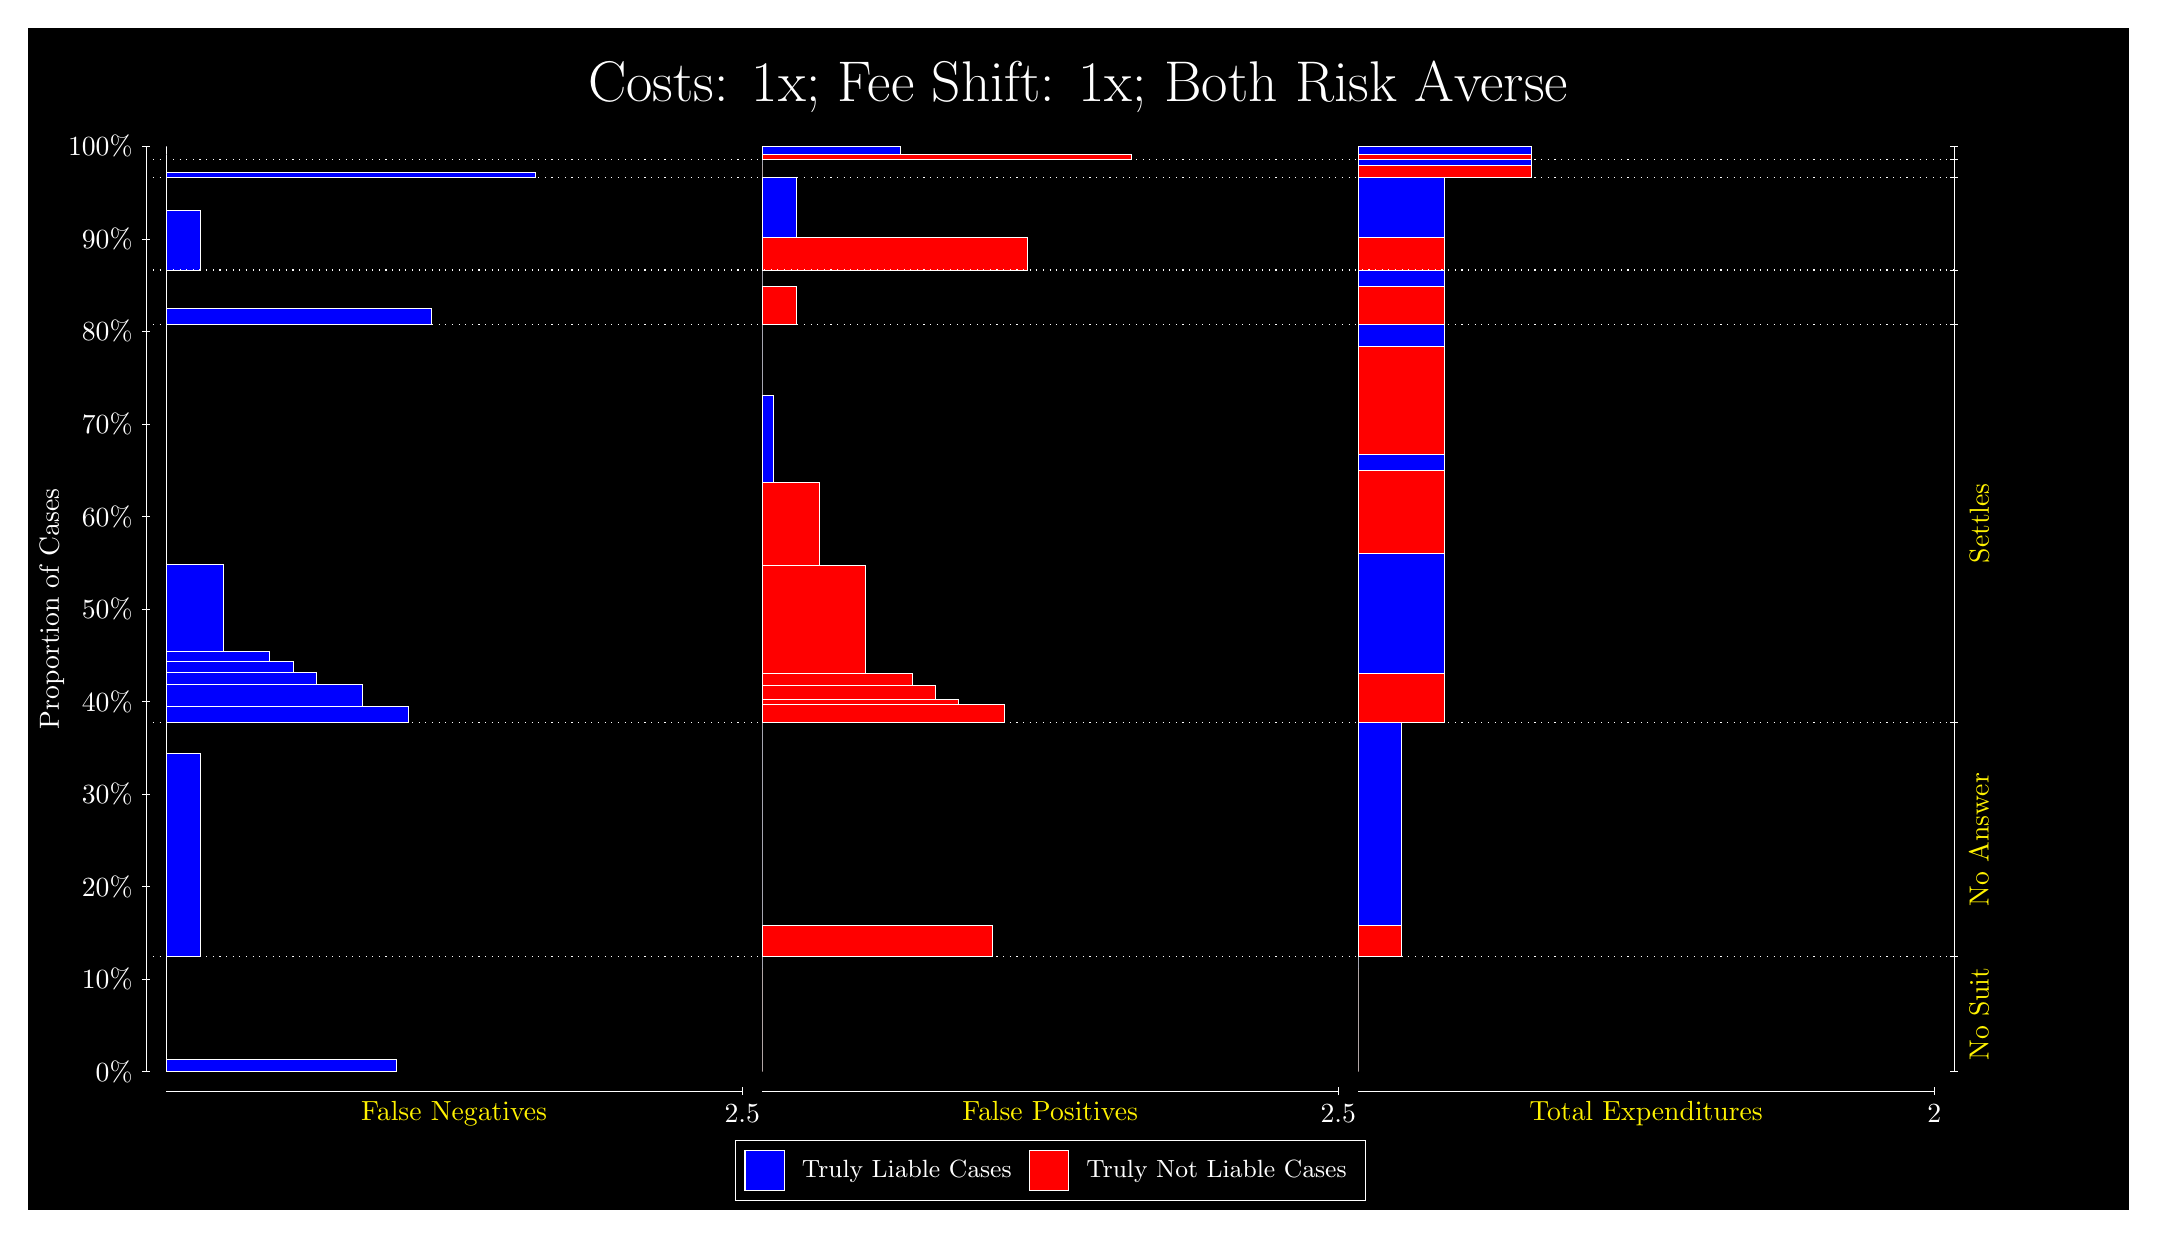
\begin{tikzpicture}
\draw[fill=black] (0,0) rectangle (26.667,15);
\draw[text=white] (0,13.5) rectangle (26.667,15) node[midway] {\huge Costs: 1x; Fee Shift: 1x; Both Risk Averse};
\draw[white, very thin] (1.5,1.75) -- (1.5,13.5);
\node[rotate=90, text=white, anchor=center] at (0.3, 7.625) {Proportion of Cases};
\draw[white, very thin] (1.45,1.75) -- (1.55,1.75);
\node[text=white, anchor=east] at (1.45, 1.75) {0\%};
\draw[white, very thin] (1.45,2.925) -- (1.55,2.925);
\node[text=white, anchor=east] at (1.45, 2.925) {10\%};
\draw[white, very thin] (1.45,4.1) -- (1.55,4.1);
\node[text=white, anchor=east] at (1.45, 4.1) {20\%};
\draw[white, very thin] (1.45,5.275) -- (1.55,5.275);
\node[text=white, anchor=east] at (1.45, 5.275) {30\%};
\draw[white, very thin] (1.45,6.45) -- (1.55,6.45);
\node[text=white, anchor=east] at (1.45, 6.45) {40\%};
\draw[white, very thin] (1.45,7.625) -- (1.55,7.625);
\node[text=white, anchor=east] at (1.45, 7.625) {50\%};
\draw[white, very thin] (1.45,8.8) -- (1.55,8.8);
\node[text=white, anchor=east] at (1.45, 8.8) {60\%};
\draw[white, very thin] (1.45,9.975) -- (1.55,9.975);
\node[text=white, anchor=east] at (1.45, 9.975) {70\%};
\draw[white, very thin] (1.45,11.15) -- (1.55,11.15);
\node[text=white, anchor=east] at (1.45, 11.15) {80\%};
\draw[white, very thin] (1.45,12.325) -- (1.55,12.325);
\node[text=white, anchor=east] at (1.45, 12.325) {90\%};
\draw[white, very thin] (1.45,13.5) -- (1.55,13.5);
\node[text=white, anchor=east] at (1.45, 13.5) {100\%};

\draw[white, very thin] (24.457,1.75) -- (24.457,13.5);
\draw[white, very thin] (24.407,1.75) -- (24.507,1.75);
\node[anchor=west] at (24.407, 1.75) {};
\draw[white, very thin] (24.407,3.2075) -- (24.507,3.2075);
\node[anchor=west] at (24.407, 3.2075) {};
\draw[white, very thin] (24.407,6.1864) -- (24.507,6.1864);
\node[anchor=west] at (24.407, 6.1864) {};
\draw[white, very thin] (24.407,11.24) -- (24.507,11.24);
\node[anchor=west] at (24.407, 11.24) {};
\draw[white, very thin] (24.407,11.93) -- (24.507,11.93);
\node[anchor=west] at (24.407, 11.93) {};
\draw[white, very thin] (24.407,13.106) -- (24.507,13.106);
\node[anchor=west] at (24.407, 13.106) {};
\draw[white, very thin] (24.407,13.33) -- (24.507,13.33);
\node[anchor=west] at (24.407, 13.33) {};
\draw[white, very thin] (24.407,13.5) -- (24.507,13.5);
\node[anchor=west] at (24.407, 13.5) {};

\draw[white, very thin, fill=blue] (1.75,1.75) rectangle (4.6775,1.9033);
\draw[white, very thin, fill=red] (1.75,1.9033) rectangle (1.75,3.2075);
\draw[white, very thin, fill=blue] (1.75,3.2075) rectangle (2.1891,5.7894);
\draw[white, very thin, fill=red] (1.75,5.7894) rectangle (1.75,6.1864);
\draw[white, very thin, fill=blue] (1.75,6.1864) rectangle (4.8239,6.3898);
\draw[white, very thin, fill=blue] (1.75,6.3898) rectangle (4.2384,6.6696);
\draw[white, very thin, fill=blue] (1.75,6.6696) rectangle (3.6529,6.8179);
\draw[white, very thin, fill=blue] (1.75,6.8179) rectangle (3.3602,6.9623);
\draw[white, very thin, fill=blue] (1.75,6.9623) rectangle (3.0674,7.0874);
\draw[white, very thin, fill=blue] (1.75,7.0874) rectangle (2.4819,8.1947);
\draw[white, very thin, fill=red] (1.75,8.1947) rectangle (1.75,11.24);
\draw[white, very thin, fill=blue] (1.75,11.24) rectangle (5.1167,11.445);
\draw[white, very thin, fill=red] (1.75,11.445) rectangle (1.75,11.93);
\draw[white, very thin, fill=blue] (1.75,11.93) rectangle (2.1891,12.687);
\draw[white, very thin, fill=red] (1.75,12.687) rectangle (1.75,13.106);
\draw[white, very thin, fill=blue] (1.75,13.106) rectangle (6.4341,13.171);
\draw[white, very thin, fill=red] (1.75,13.171) rectangle (1.75,13.33);
\draw[white, very thin, fill=red] (1.75,13.33) rectangle (1.75,13.395);
\draw[white, very thin, fill=blue] (1.75,13.395) rectangle (1.75,13.5);
\draw[white, very thin, fill=red] (9.3189,1.75) rectangle (9.3189,3.0542);
\draw[white, very thin, fill=blue] (9.3189,3.0542) rectangle (9.3189,3.2075);
\draw[white, very thin, fill=red] (9.3189,3.2075) rectangle (12.246,3.6045);
\draw[white, very thin, fill=blue] (9.3189,3.6045) rectangle (9.3189,6.1864);
\draw[white, very thin, fill=red] (9.3189,6.1864) rectangle (12.393,6.4195);
\draw[white, very thin, fill=red] (9.3189,6.4195) rectangle (11.807,6.4761);
\draw[white, very thin, fill=red] (9.3189,6.4761) rectangle (11.515,6.6565);
\draw[white, very thin, fill=red] (9.3189,6.6565) rectangle (11.222,6.8047);
\draw[white, very thin, fill=red] (9.3189,6.8047) rectangle (10.636,8.1796);
\draw[white, very thin, fill=red] (9.3189,8.1796) rectangle (10.051,9.2321);
\draw[white, very thin, fill=blue] (9.3189,9.2321) rectangle (9.4652,10.339);
\draw[white, very thin, fill=blue] (9.3189,10.339) rectangle (9.3189,11.24);
\draw[white, very thin, fill=red] (9.3189,11.24) rectangle (9.758,11.725);
\draw[white, very thin, fill=blue] (9.3189,11.725) rectangle (9.3189,11.93);
\draw[white, very thin, fill=red] (9.3189,11.93) rectangle (12.686,12.349);
\draw[white, very thin, fill=blue] (9.3189,12.349) rectangle (9.758,13.106);
\draw[white, very thin, fill=red] (9.3189,13.106) rectangle (9.3189,13.265);
\draw[white, very thin, fill=blue] (9.3189,13.265) rectangle (9.3189,13.33);
\draw[white, very thin, fill=red] (9.3189,13.33) rectangle (14.003,13.395);
\draw[white, very thin, fill=blue] (9.3189,13.395) rectangle (11.075,13.5);
\draw[white, very thin, fill=red] (16.888,1.75) rectangle (16.888,3.0542);
\draw[white, very thin, fill=blue] (16.888,3.0542) rectangle (16.888,3.2075);
\draw[white, very thin, fill=red] (16.888,3.2075) rectangle (17.437,3.6045);
\draw[white, very thin, fill=blue] (16.888,3.6045) rectangle (17.437,6.1864);
\draw[white, very thin, fill=red] (16.888,6.1864) rectangle (17.986,6.8047);
\draw[white, very thin, fill=blue] (16.888,6.8047) rectangle (17.986,8.3298);
\draw[white, very thin, fill=red] (16.888,8.3298) rectangle (17.986,9.3823);
\draw[white, very thin, fill=blue] (16.888,9.3823) rectangle (17.986,9.5857);
\draw[white, very thin, fill=red] (16.888,9.5857) rectangle (17.986,10.961);
\draw[white, very thin, fill=blue] (16.888,10.961) rectangle (17.986,11.24);
\draw[white, very thin, fill=red] (16.888,11.24) rectangle (17.986,11.725);
\draw[white, very thin, fill=blue] (16.888,11.725) rectangle (17.986,11.93);
\draw[white, very thin, fill=red] (16.888,11.93) rectangle (17.986,12.349);
\draw[white, very thin, fill=blue] (16.888,12.349) rectangle (17.986,13.106);
\draw[white, very thin, fill=red] (16.888,13.106) rectangle (19.083,13.265);
\draw[white, very thin, fill=blue] (16.888,13.265) rectangle (19.083,13.33);
\draw[white, very thin, fill=red] (16.888,13.33) rectangle (19.083,13.395);
\draw[white, very thin, fill=blue] (16.888,13.395) rectangle (19.083,13.5);
\draw[white, dotted] (1.5,3.2075) -- (24.457,3.2075);
\draw[white, dotted] (1.5,6.1864) -- (24.457,6.1864);
\draw[white, dotted] (1.5,11.24) -- (24.457,11.24);
\draw[white, dotted] (1.5,11.93) -- (24.457,11.93);
\draw[white, dotted] (1.5,13.106) -- (24.457,13.106);
\draw[white, dotted] (1.5,13.33) -- (24.457,13.33);
\draw[white, very thin] (1.75,1.5) -- (9.0689,1.5);
\node[text=yellow, anchor=north] at (5.4094, 1.5) {False Negatives};
\draw[white, very thin] (9.0689,1.45) -- (9.0689,1.55);
\node[text=white, anchor=north] at (9.0689, 1.45) {2.5};

\draw[white, very thin] (9.3189,1.5) -- (16.638,1.5);
\node[text=yellow, anchor=north] at (12.978, 1.5) {False Positives};
\draw[white, very thin] (16.638,1.45) -- (16.638,1.55);
\node[text=white, anchor=north] at (16.638, 1.45) {2.5};

\draw[white, very thin] (16.888,1.5) -- (24.207,1.5);
\node[text=yellow, anchor=north] at (20.547, 1.5) {Total Expenditures};
\draw[white, very thin] (24.207,1.45) -- (24.207,1.55);
\node[text=white, anchor=north] at (24.207, 1.45) {2};

\node[text=yellow, centered, rotate=90] at (24.777, 2.4788) {No Suit};
\node[text=yellow, centered, rotate=90] at (24.777, 4.697) {No Answer};
\node[text=yellow, centered, rotate=90] at (24.777, 8.7134) {Settles};





\draw (12.978300999999998,1.5) node[draw=none] (baseCoordinate) {};
\begin{scope}[align=center]
        \matrix[scale=0.5, draw=white, below=0.5cm of baseCoordinate, nodes={draw}, column sep=0.1cm]{
            \node[rectangle, draw, minimum width=0.5cm, minimum height=0.5cm, fill=blue] {}; &
            \node[draw=none, font=\small, text=white] (B) {Truly Liable Cases}; &
            \node[rectangle, draw, minimum width=0.5cm, minimum height=0.5cm, fill=red] {}; &
            \node[draw=none, font=\small, text=white] (B) {Truly Not Liable Cases}; \\
            };
\end{scope}

\end{tikzpicture}
\end{document}